\subsection{Adding Constraints to the Solver}
\label{subsec:constraint}

\if 0 
As we will see in \S\ref{sec:modelling_macro}, 
when the system of liner equations suffers the two conditions above, the regression solver may output different solutions that all minimize the fitting error, which may violate basic properties of the power model parameter values. To overcome this, in addition to the basic unconstrained solver, 
\fi 
We experimented with adopting two ways for constraining the solutions generated by the regression solver based on simple domain knowledge, as shown in Table~\ref{tab:constrained}.

\begin{table}[tp]
%\questionaj{These constraints must also constrain GPU busy and idle.}
{\small
    \centering
    \caption{Constraints added to the regression solver.}
    \vspace{-0.1in}
    \begin{tabular}{|p{25mm}|p{52mm}|}
    \hline
         Constrainted SPMD  & \multicolumn{1}{c|}{Description} \\
         \hline
         Unconstrained      & No constraints are applied. \\
         Constrained        & Model parameters should not decrease with increasing frequencies. GPU idle power is less than Budy power. \\
         Freq-constrained   & CPU model parameters are modeled as a polynomial of frequency. \\
         \hline
    \end{tabular}
    \label{tab:constrained}
    \vspace{-0.1in}
}
\end{table}


\paragraph{Constraint 1: positivity and monotonicity}
Without any constraint, we found the regression solver can output CPU/GPU power values those are negative or 
decreasing while the frequency increases.
To prevent the solver from outputing such solutions, we add three constraints to the regression solver: 
(1) all model parameters should be positive;
(2) the model parameters with increasing frequencies for each component should be non-decreasing;
(3) the GPU Idle power should be lower than the GPU Busy power. 
We denote this version of SPMD as "Constrained SPMD" in Table~\ref{tab:constrained}.


\paragraph{Constraint 2: modeling CPU power as a function of frequency}
We found even with Constraint 1, the 
CPU power parameters output by the solver often does not change with varying frequencies. 
To make the CPU model parameters output more consistent with the reality, 
we exploited another domain knowledge about the CPU power draw,
that the power draw increases as per a low-order polynomial of the operating frequency~\cite{armdvfs,rizvandi2011some}.
% Since the specific polynomial function may vary for different phones, \eg early phones only performed % frequency scaling (FS) while newer phones perform dynamic voltage and frequency scaling (DVFS), we first used a simple CPU benchmark to find the order of the polynomial for each phone used in our experiments. 
%
\if 0
\begin{figure}[tp]
    \centering
%    \vspace{-0.1in}
    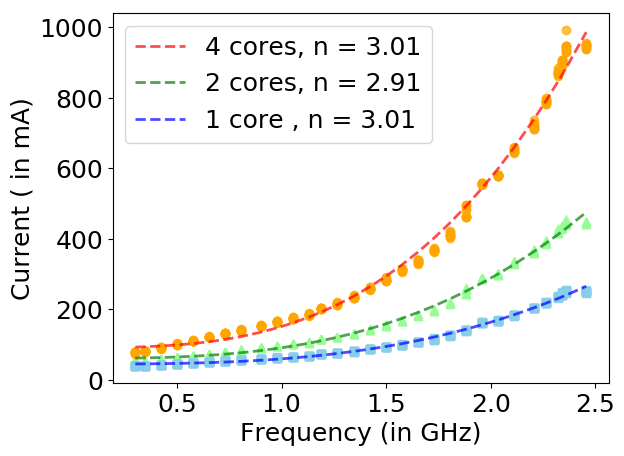
\includegraphics[width=0.80\columnwidth]{figures/cpu_characteristics.png}
    \caption{Moto Z3 big core CPU power draw grows with frequency 
    when running the arithmetic-intensive benchmark.}
    \label{fig:cpu_characteristic}
    \vspace{-0.1in}
\end{figure}
\fi
%
\cut{ We ran a microbenchmark that performs arithmetic-intensive or memory-intensive operations for 7 seconds
on 1, 2 and 4 big cores, for each big core frequency, and fit the measured phone power 
with a polynomial function in frequency.
%\begin{equation}
%     P_{CPU} = p^c_{base}+ \sum_i p^c_i({f_k}) = p_{base}+\sum_i  a*f_k^{n}
% \end{equation}
% Figure~\ref{fig:cpu_characteristic} shows the measured power draw and curve fitting on Moto Z3.
}
Our CPU microbenchmark results show show that 
% the fitted exponent $n$ for 1, 2 and 4 cores are 3.01, 2.97 and 3.01, respectively.
the per core power of Moto Z3 grows as the third-power of the CPU frequency.
Thus we replace all the CPU power parameters with third-power of the CPU frequency in the SPMD model equations.
%model the Moto Z3 big core power as a third-order polynomial of the CPU frequency in the model equations of SPMD.
%
Doing so has two benefits: (1) it reduces the number of CPU power parameters from $K$ - the number of CPU frequencies - to 2, $p_{base}$ and coefficient $a$, which reduces the number of equations needed for the solver; (2) it puts constraints for the CPU power  to be not only  monotonic, but consistent with physics.
